\documentclass[12pt,notes]{beamer}

\usecolortheme[dark,accent=yellow]{solarized}
\beamertemplatetransparentcovered
\setbeamertemplate{navigation symbols}{} % remove navigation symbols
% \setbeamertemplate{footline}[page number]
\setbeamertemplate{footline}{
  \hfill%
  \usebeamercolor[fg]{page number in head/foot}%
  \usebeamerfont{page number in head/foot}%
  \setbeamertemplate{page number in head/foot}[framenumber]%
  \usebeamertemplate*{page number in head/foot}\kern1em\vskip2pt%
}
\setbeamerfont{page number in head/foot}{size=\small}
\setbeamerfont{note page}{size=\scriptsize}

\usepackage[german]{babel}
\usepackage{times}
\usepackage{esvect}\renewcommand{\vec}[1]{\vv{#1}}
\usepackage{setspace}\setstretch{1.5}
\usepackage{tikz}
\usepackage{pgfplots}\pgfplotsset{compat=1.17}
\usepackage{siunitx}
\usepackage{multimedia}

%%%%%%%%%%%%%%%%%%%%%%%%%%%%%%%%%%%%%%%%%%%%%%%%%%

\usetikzlibrary{calc,decorations.markings,decorations.pathmorphing,positioning,shapes}

% default arrow style
\tikzset{>=latex}

\tikzset{photon/.style={decorate, decoration={snake, segment length=2mm, amplitude=1mm}}}

\tikzset{%
    ->-/.style={postaction={decorate},decoration={%
            markings,mark=at position #1 with {\arrow{>}}%
        }%
    },%
    ->-/.default=.5,%
    -<-/.style={postaction={decorate},decoration={%
            markings,mark=at position #1 with {\arrowreversed{>}}%
        }%
    },%
    -<-/.default=.5%
}

% arrows on the field lines
\tikzstyle directed=[postaction={decorate,decoration={markings,
  mark=at position .2 with {\arrowreversed[scale=1.5]{>}},
  mark=at position .8 with {\arrowreversed[scale=1.5]{>}}}}]

% field lines
\tikzstyle fLines=[thick,directed]

\newcommand{\magnet}[3]{%
    \def\lmag{#1}  % length of magnet
    \def\wmag{#2}  % thickness of magnet
    \def\nc{#3}    % no. of lines = 2*\nc+1
    \begin{scope}
      \coordinate (A) at (-\lmag/2,\wmag/2);
      \coordinate (B) at (\lmag/2,-\wmag/2);
      \draw[fill, color=green](A) rectangle ++(\lmag/2,-\wmag) node[black,midway]{S};
      \draw[fill, color=red](0,-\wmag/2) rectangle ++(\lmag/2,\wmag) node[black,midway]{N};
      \clip (-5,-3) rectangle (5,3);
      \foreach \r in {1,...,\nc}{
        \draw[fLines]($(A)-(0,0.5*\r*\wmag/\nc)$) arc(({270-asin(\lmag/(2*\r))}):({-90+asin(\lmag/(2*\r))}):\r);
        \draw[fLines]($(B)+(0,0.5*\r*\wmag/\nc)$) arc(({90-asin(\lmag/(2*\r))}):({-270+asin(\lmag/(2*\r))}):\r); }
      \draw[fLines] (-\lmag/2,0) -- ++(-6,0);
      \draw[fLines] (\lmag/2,0) ++(6,0)--(\lmag/2,0);
    \end{scope}
    \draw[blue,->,line width=3] (-\nc/8,2) -- ++(\nc/4,0) node[midway,above] {$\vec{m}$};
}

% Quantum correction, #1 = coordinate for origin, #2 = angle
\newcommand{\QC}[2]{%
  \begin{scope}[shift={#1},rotate around={#2:(0,0)}]
    % \draw[blue,fill] (0,0) circle (0.05);
    % \draw[blue,fill] (1,0) circle (0.05);
    \pgfmathsetmacro{\angl}{45}
    \draw[->-=0.7,blue] (0,0) to[out={-\angl},in={180+\angl}] node[pos=0.3,green] (a) {} (1,0);
    \draw[->-=0.7,blue] (0,0) to[out={\angl}, in={90+\angl}]  node[pos=0.3,green] (b) {} (1,0);
    \draw[green,fill] (a) circle (0.05);
    \draw[green] (b) circle (0.05);
  \end{scope}
}

\newcommand{\SMtable}{%
    \begin{tikzpicture}[node distance = 2.5em, auto]
      \node[quark] (u) {$u$};
      \node[quark, below of=u] (d) {$d$};
      \node[quark, right of=u] (c) {$c$};
      \node[quark, below of=c] (s) {$s$};
      \node[quark, right of=c] (t) {$t$};
      \node[quark, below of=t] (b) {$b$};
      \node[lepton, below of=d] (ne) {$\nu_e$};
      \node[lepton, below of=ne] (e) {$e$};
      \node[lepton, right of=ne] (nm) {$\nu_\mu$};
      \node[lepton, below of=nm] (m) {$\mu$};
      \node[lepton, right of=nm] (nt) {$\nu_\tau$};
      \node[lepton, below of=nt] (ta) {$\tau$};
      \node[gauge, right of=t] (gamma) {$\gamma$};
      \node[gauge, below of=gamma] (g) {$g$};
      \node[gauge, below of=g] (Z) {$Z$};
      \node[gauge, below of=Z] (W) {$W$};
      \node[scalar, right of=W] (H) {$h$};
      \node[rotate=90] (quarks)  at ($(u)!0.5!(d)+(-1,0)$)  {quarks};
      \node[rotate=90] (leptons) at ($(ne)!0.5!(e)+(-1,0)$) {leptons};
      \node[below of=H] (higgs) {Higgs};
      \node[above of=gamma, align=center] (gauge) {gauge\\[-0.5em] bosons};
    \end{tikzpicture}
}

%%%%%%%%%%%%%%%%%%%%%%%%%%%%%%%%%%%%%%%%%%%%%%%%%%

\tikzstyle{block} = [rectangle, draw, text width=7em, text centered, minimum height=2em]

\tikzstyle{quark}     = [rectangle, black, draw, fill=yellow, minimum width=2em, text centered, minimum height=2em]
\tikzstyle{lepton}    = [rectangle, black, draw, fill=red!50, minimum width=2em, text centered, minimum height=2em]
\tikzstyle{gauge}     = [circle   , black, draw, fill=green , minimum size=2em, inner sep=0pt, text centered]
\tikzstyle{scalar}    = [diamond  , black, draw, fill=blue!40, minimum width=2.3em, text centered, minimum height=2.3em, inner sep=0pt]
\tikzstyle{goldstone} = [diamond  , black, draw, dashed, fill=blue!30, minimum width=2.3em, text centered, minimum height=2.3em, inner sep=0pt]
\tikzstyle{squark}    = [diamond  , black, draw, fill=yellow, minimum width=2.3em, text centered, minimum height=2.3em, inner sep=0pt]
\tikzstyle{slepton}   = [diamond  , black, draw, fill=red!50, minimum width=2.3em, text centered, minimum height=2.3em, inner sep=0pt]
\tikzstyle{gaugino}   = [rectangle, black, draw, fill=green , minimum size=2em, inner sep=0pt, text centered]
\tikzstyle{higgsino}  = [rectangle, black, draw, fill=blue!40  , minimum width=2em, text centered, minimum height=2em]
\tikzstyle{inert}     = [diamond  , black, draw, fill=teal!80, minimum width=2.3em, text centered, minimum height=2.3em, inner sep=0pt]
\tikzstyle{inertino}  = [rectangle, black, draw, fill=teal!80, minimum width=2em, text centered, minimum height=2em]
\tikzstyle{phantom}   = [rectangle, black, minimum width=2em, text centered, minimum height=2em]

%%%%%%%%%%%%%%%%%%%%%%%%%%%%%%%%%%%%%%%%%%%%%%%%%%

\newcommand{\Exp}{\text{Exp}}
\newcommand{\SM}{\text{SM}}

% BNL-E821
\newcommand{\amuBNL}{11659209.1} % 
\newcommand{\numamuBNL}{\num{\amuBNL}}
\newcommand{\DamuBNL}{6.3}

% FNAL 2021
\newcommand{\amuFNAL}{11659204.0}
\newcommand{\DamuFNAL}{5.4}
\newcommand{\numamuFNAL}{\num{\amuFNAL}}

% experimental, combined
\newcommand{\amuExp}{11659206.1}
\newcommand{\numamuExp}{\num{\amuExp}}
\newcommand{\DamuExp}{4.1} % uncertainty
\newcommand{\aeExp}{11596521807.3}
\newcommand{\numaeExp}{\num{\aeExp}}
\newcommand{\DaeExp}{2.8}

% SM
\newcommand{\amuSM}{11659181.0}
\newcommand{\numamuSM}{\num{\amuSM}}
\newcommand{\DamuSM}{4.3}
\newcommand{\aeSM}{11596521816.4}
\newcommand{\numaeSM}{\num{\aeSM}}
\newcommand{\DaeSM}{7.7}

\definecolor{red}{rgb}{1.0,0.2,0.2}
\definecolor{blue}{rgb}{0,0.7,1.0}
\definecolor{green}{rgb}{0,1.0,0.5}

%%%%%%%%%%%%%%%%%%%%%%%%%%%%%%%%%%%%%%%%%%%%%%%%%%

\title{The magic is always in the details}
\subtitle{The search for new physics with the muon}

\author[Voigt]{Alexander Voigt}
\institute[HS Flensburg]{Hochschule Flensburg}
\date{Planetarium Talks 2022}

\begin{document}

%%%%%%%%%%%%%%%%%%%%%%%%%%%%%%%%%%%%%%%%%%%%%%%%%%

\begin{frame}
  \titlepage
\end{frame}

%%%%%%%%%%%%%%%%%%%%%%%%%%%%%%%%%%%%%%%%%%%%%%%%%%

\begin{frame}{Table of Contents}
  \tableofcontents
\end{frame}

%%%%%%%%%%%%%%%%%%%%%%%%%%%%%%%%%%%%%%%%%%%%%%%%%%

\section{Introduction}

\begin{frame}{}
  \begin{center}
    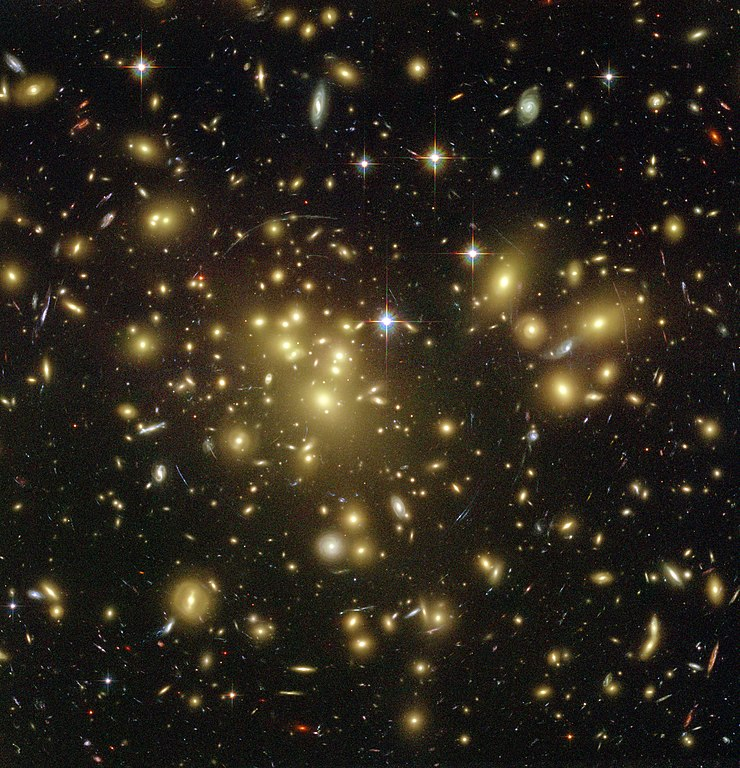
\includegraphics[width=0.8\textwidth]{img/Gravitationell-lins-Hubble}

    \hfill\footnotesize [Abell 1689, ESA/Hubble]
  \end{center}
\end{frame}

\note{
  \begin{itemize}
  \item Start with picture of the galaxy cluster ``Abell 1689'' from the Hubble telescope
  \item look closely: you'll see a gravity lens effect
  \item So, there must be some massive object(s) between the galaxy
    cluster and us
  \item If one counts the number of visible objects (stars), one finds
    that (assuming ART is correct), the cumulative mass of the stars
    is not enough to explain this gravity lens effect.
  \item So, there must be some invisible massive matter between the
    galaxy cluster and us. This is what astronomers and cosmologists
    call ``Dark Matter''.
  \end{itemize}
}

\begin{frame}{}
  \begin{center}
    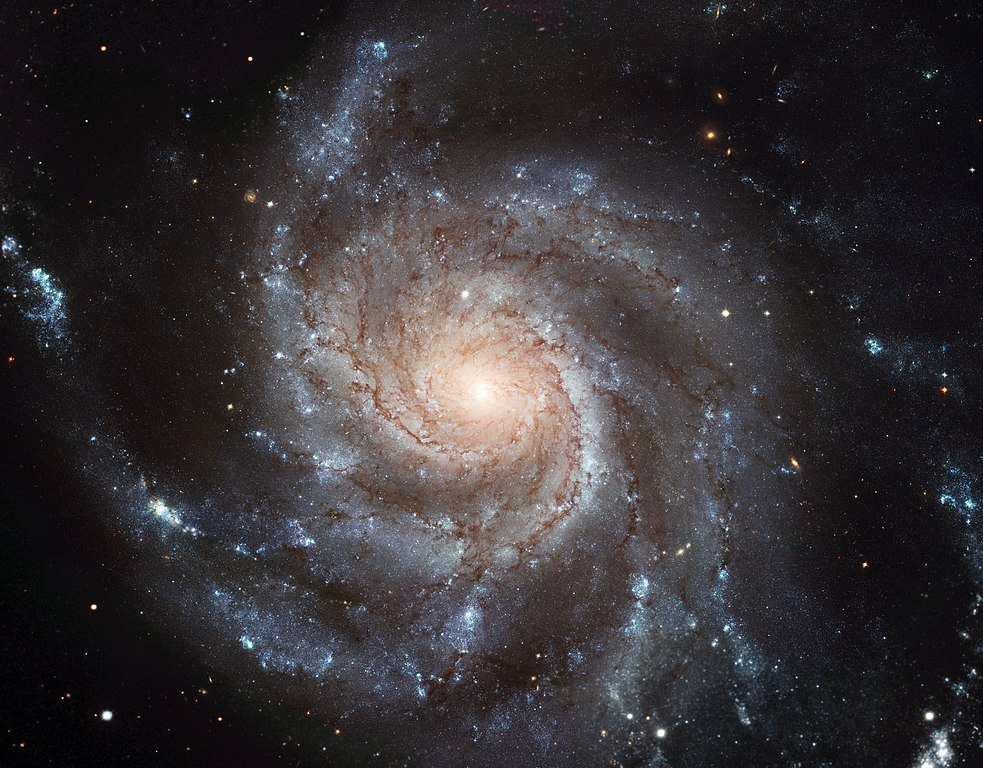
\includegraphics[width=0.8\textwidth]{img/Galaxy-M101}

    \hfill\footnotesize [ESA/Hubble]
  \end{center}
\end{frame}

\note{
  \begin{itemize}
  \item Look at the photo from the Hubble telescope, it shows a spiral
    galaxy, which is rotating.
  \item If one counts the number of (visible) stars, one can estimate
    the mass distribution of the galaxy.
  \item From the mass distribution, one can predict (using ART) the
    speed at which the outer stars move around the center.
  \item However, one finds that the speed tends to be significantly
    larger than expected.
  \item This effect could be explained if there would be some
    invisible (Dark Matter) that fills the galaxy.
  \end{itemize}
}

\begin{frame}{}
  \begin{center}
    \movie[width=\textwidth,autostart,loop]{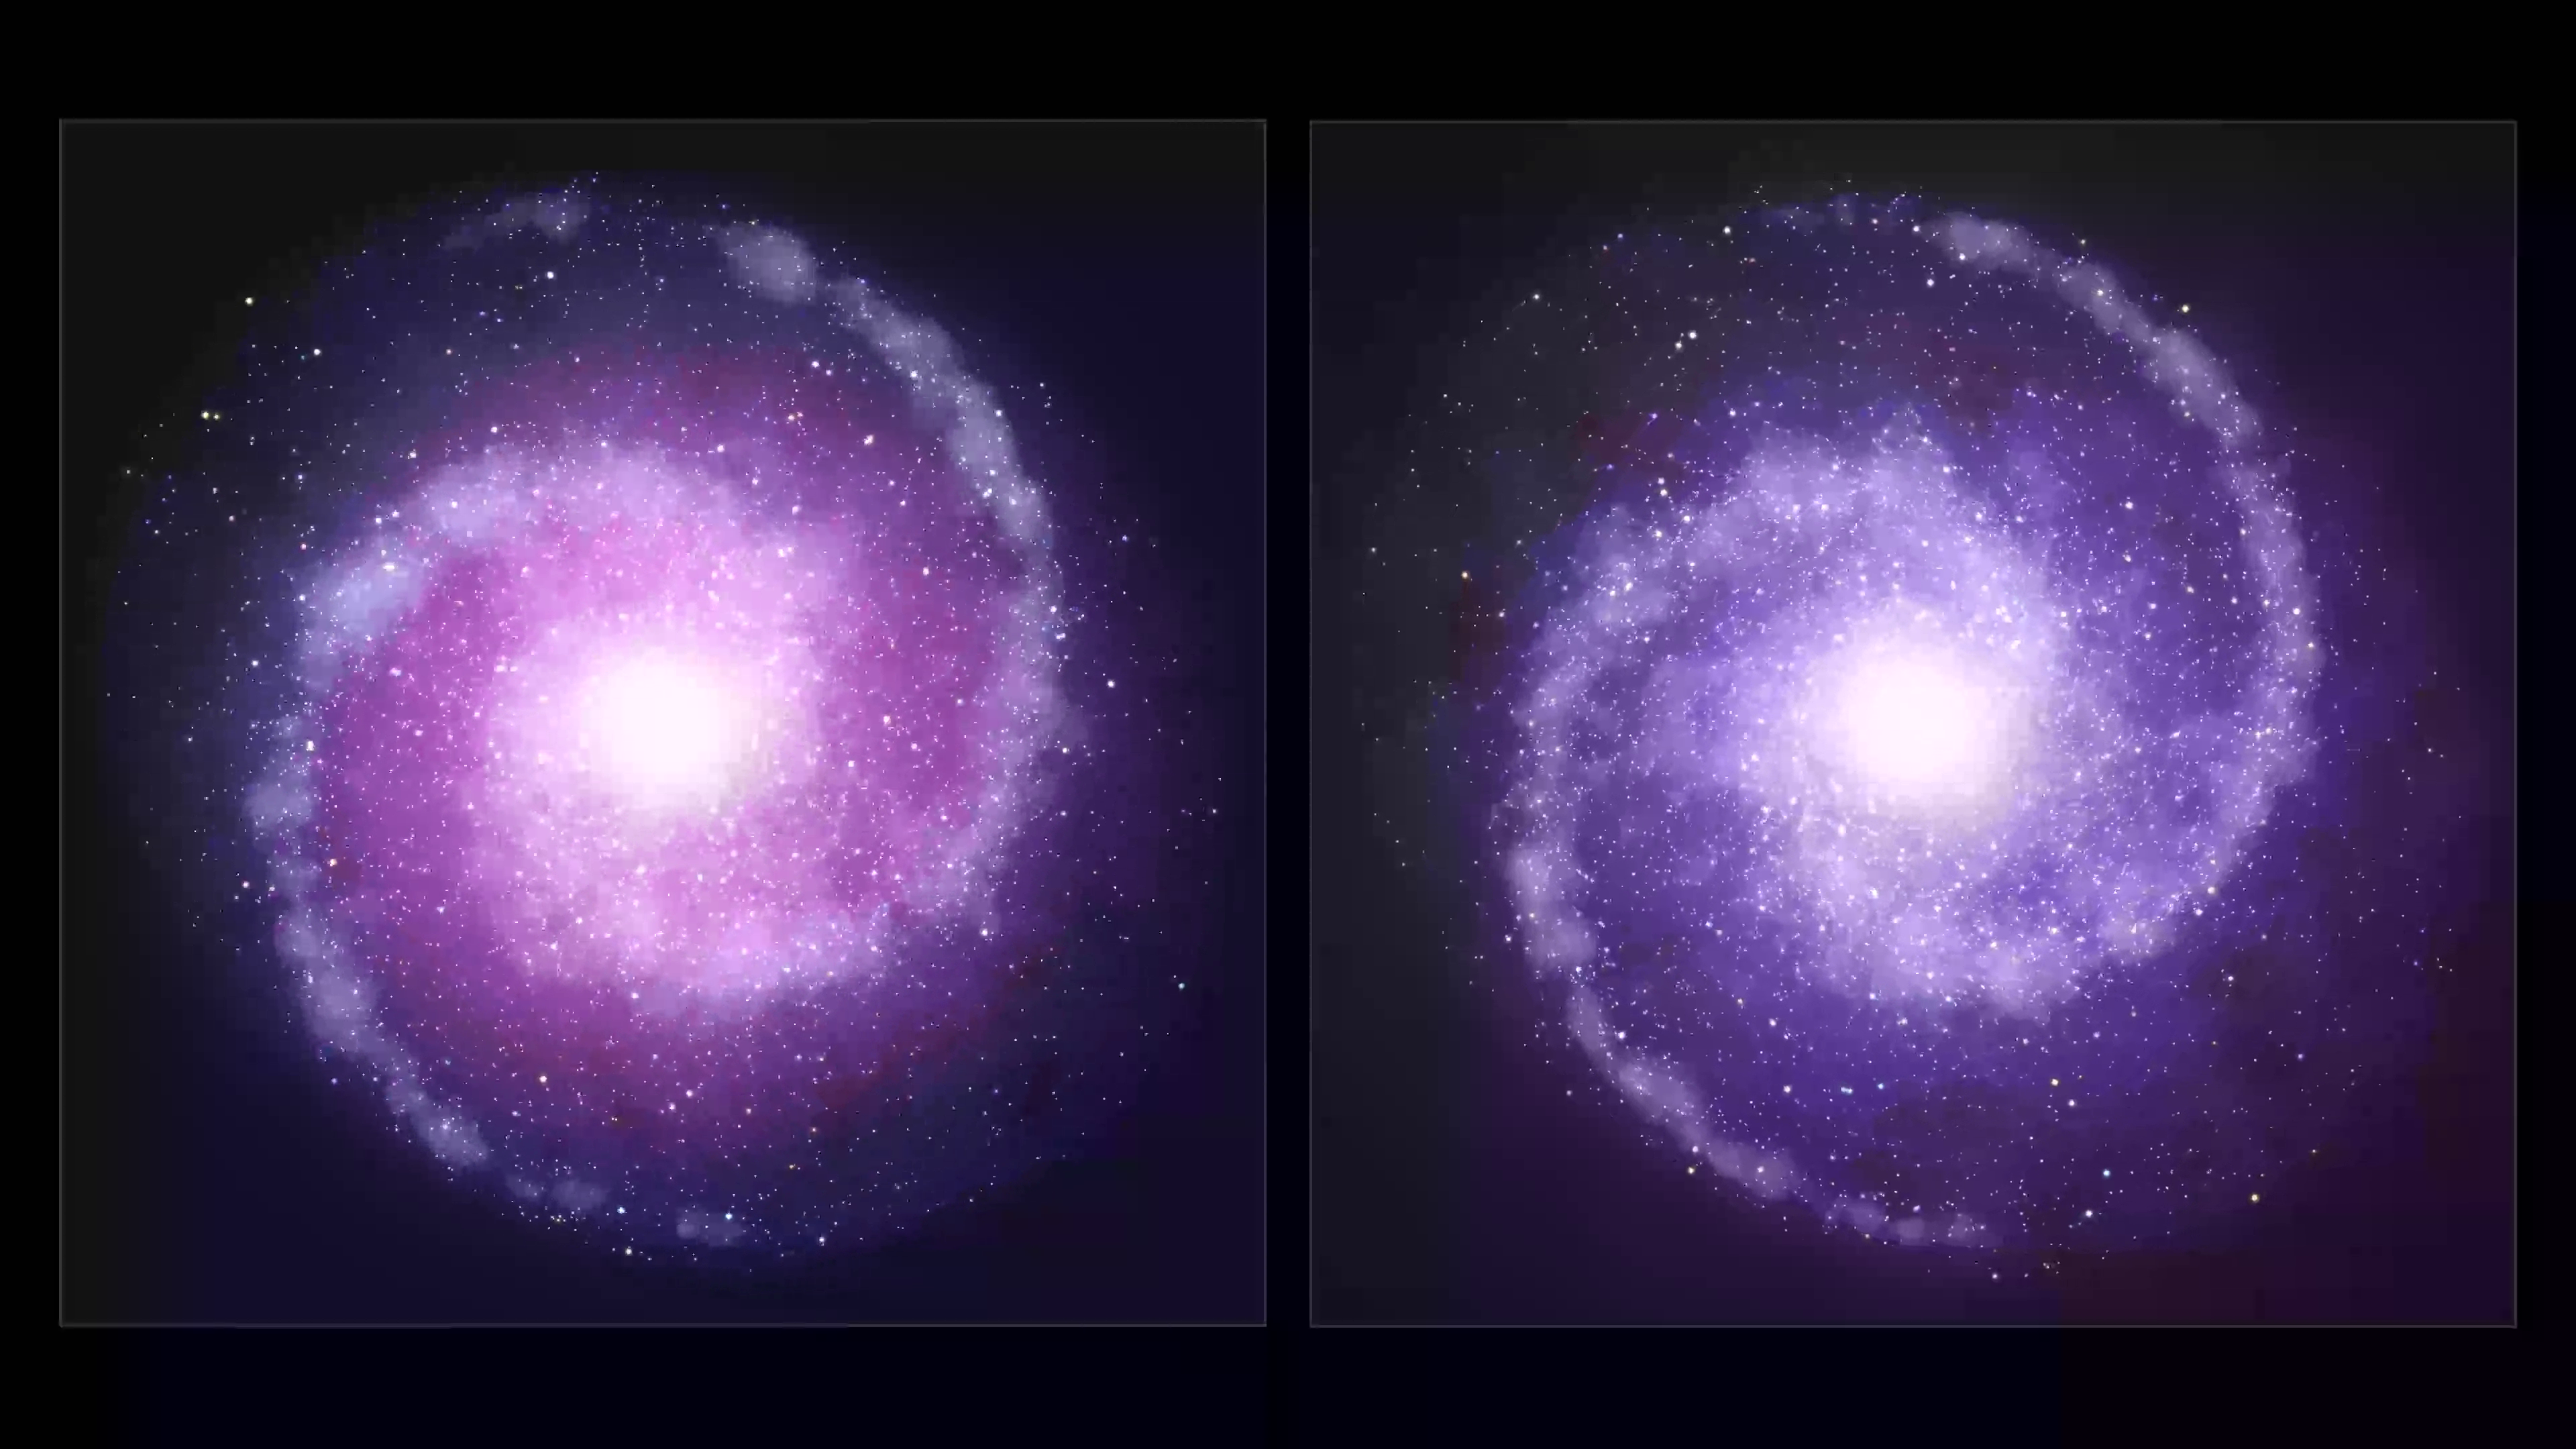
\includegraphics[width=\textwidth]{videos/dark_matter_affecting_galaxy_rotation.png}}{videos/dark_matter_affecting_galaxy_rotation.webm}
  \end{center}
\end{frame}

%%%%%%%%%%%%%%%%%%%%%%%%%%%%%%%%%%%%%%%%%%%%%%%%%%

\section{Magnetism}

\begin{frame}{\insertsection}
  \begin{center}
    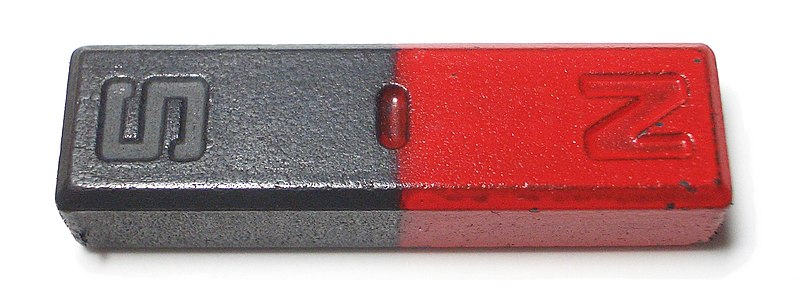
\includegraphics[width=0.9\textwidth]{img/bar_magnet_foto}

    \hfill\footnotesize [Aney, CC-SA-3.0]
  \end{center}
\end{frame}

\note{
  \begin{itemize}
  \item In the following I'll describe one interesting pheomenon,
    which may be one possibility to shed light on the origin of Dark
    Matter.
  \item The phenomenon is called the ``anomalous magnetic moment''.
  \item This phenomenon has to do with plain magnetism.
  \item To explain what the magnetic moment is, lets start looking at
    a conventional solid magnet (paramagnetism or ferromagnetism).
  \end{itemize}
}

\begin{frame}{\insertsection: magnetic moment $\vec{m}$}
  \begin{tikzpicture}
    \only<1>{\magnet{1.8}{0.5}{3}}%
    \only<2>{\magnet{1.8}{0.5}{4}}%
    \only<3>{\magnet{1.8}{0.5}{5}}%
    \only<4>{\magnet{1.8}{0.5}{6}}%
    \only<5>{\magnet{1.8}{0.5}{7}}%
    \only<6>{\magnet{1.8}{0.5}{8}}%
    \only<7>{\magnet{1.8}{0.5}{9}}%
    \only<8>{\magnet{1.8}{0.5}{10}}%
    \only<9>{\magnet{1.8}{0.5}{11}}%
  \end{tikzpicture}  
\end{frame}

\note{
  \begin{itemize}
  \item This solid magnet has a magnetic field, which can be
    visualized with magnetic field lines (gray).
  \item If one would bring another magnet close to this magnet, the
    magnet would start experience a torque (Drehmoment).
  \item To describe the torque that the magnet experiences, one
    assigns a vector to the magnet, called the ``magnetic dipole
    moment'' $\vec{m}$ (blue).
  \item The magnetic dipole moment $\vec{m}$ of this shown magnet
    points from its south pole to its north pole.
  \item The magnitude of the magnetic dipole moment $\vec{m}$ (i.e.\
    the length of the vector) is a measure for the ``strength'' of the
    magnetic field.
  \end{itemize}
}

% \begin{frame}{\insertsection}
%   Magnetisches Moment $\vec{m}$:
%   \begin{itemize}
%   \item Beschreibt WW eines magnetischen Dipols mit einem Magnetfeld
%   \item Betrag: "`Stärke der WW"'
%   \item Richtung: Angestrebte Ausrichtung zum Magnetfeld
%   \end{itemize}
%   Ursache des Magnetismus bei einem Permanentmagneten:
%   \begin{itemize}
%   \item Bahndrehimpuls
%   \item Spin
%   \end{itemize}
%   der Atome
% \end{frame}

\begin{frame}{\insertsection: origin}
  \begin{center}
    \begin{tikzpicture}
      \def\lmag{1.8}  % length of magnet
      \def\wmag{0.5}  % thickness of magnet
      \coordinate (A) at (-\lmag/2,\wmag/2);
      \coordinate (B) at (\lmag/2,-\wmag/2);
      \draw[fill, color=green](A) rectangle ++(\lmag/2,-\wmag) node[black,midway]{S};
      \draw[fill, color=red](0,-\wmag/2) rectangle ++(\lmag/2,\wmag) node[black,midway]{N};
    \end{tikzpicture}
  \end{center}
\end{frame}

\note{
  \begin{itemize}
  \item In order to understand the origin of the magnetic moment, we
    must look closer into the magnet.
  \end{itemize}
}

\begin{frame}{\insertsection: origin}
  \begin{center}
    \begin{tikzpicture}
      \def\lmag{4}  % length of magnet
      \def\wmag{1}  % thickness of magnet
      \coordinate (A) at (-\lmag/2,\wmag/2);
      \coordinate (B) at (\lmag/2,-\wmag/2);
      \draw[fill, color=green](A) rectangle ++(\lmag/2,-\wmag) node[black,midway]{\large S};
      \draw[fill, color=red](0,-\wmag/2) rectangle ++(\lmag/2,\wmag) node[black,midway]{\large N};
      %
      \foreach \X in {-1.9,-1.7,...,1.9} {%
        \foreach \Y in {-0.4,-0.2,...,0.4} {%
          \draw[fill,black] (\X,\Y) circle (0.01);
        }
      }
    \end{tikzpicture}
  \end{center}
\end{frame}

\begin{frame}{\insertsection: origin}
  \begin{center}
    \begin{tikzpicture}
      \def\lmag{8}  % length of magnet
      \def\wmag{2}  % thickness of magnet
      \coordinate (A) at (-\lmag/2,\wmag/2);
      \coordinate (B) at (\lmag/2,-\wmag/2);
      \draw[fill, color=green](A) rectangle ++(\lmag/2,-\wmag) node[black,midway]{\Huge S};
      \draw[fill, color=red](0,-\wmag/2) rectangle ++(\lmag/2,\wmag) node[black,midway]{\Huge N};
      %
      \foreach \X in {-3.8,-3.4,...,3.9} {%
        \foreach \Y in {-0.8,-0.4,...,0.9} {%
          \draw[fill,black] (\X,\Y) circle (0.02);
        }
      }
    \end{tikzpicture}
  \end{center}
\end{frame}

\note{
  \begin{itemize}
  \item We see that the magnet consists of atoms.
  \end{itemize}
}

\begin{frame}{\insertsection: origin}
  \begin{center}
    \begin{tikzpicture}
      \def\lmag{8}  % length of magnet
      \def\wmag{2}  % thickness of magnet
      \coordinate (A) at (-\lmag/2,\wmag/2);
      \coordinate (B) at (\lmag/2,-\wmag/2);
      \draw[fill, color=green](A) rectangle ++(\lmag/2,-\wmag) node[black,midway]{\Huge S};
      \draw[fill, color=red](0,-\wmag/2) rectangle ++(\lmag/2,\wmag) node[black,midway]{\Huge N};
      %
      \foreach \X in {-3.8,-3.4,...,3.9} {%
        \foreach \Y in {-0.8,-0.4,...,0.9} {%
          % \draw[fill,black] (\X,\Y) circle (0.02);
          \draw[black,->] (\X-0.1,\Y) -- ++(0.2,0);
        }
      }
    \end{tikzpicture}
  \end{center}
\end{frame}

\note{
  \begin{itemize}
  \item If we look at the atoms further, we find that each atom has a
    magnetic moment.
  \item The magnetic moments of all atoms together make up the total
    magnetic moment of the magnet.
  \end{itemize}
}

\begin{frame}{\insertsection: origin}
  \begin{center}
    \begin{tikzpicture}
      \fill[even odd rule,inner color=blue,outer color=solarizedRebase03!100] (0,0) circle (3);
      \coordinate (n) at (0,0);
      \coordinate (e) at (2,0.5);
      \draw[fill,red] (n) circle (0.1);
      \draw[fill,green] (e) circle (0.05);
      \only<1>{%
        \node[below,black] at (n) {nucleus};
        \node[below,green] at (e) {electron};
      }%
      \only<2>{%
        \draw[very thick,red,->] ($(n)+(0,-1)$) -- ++(0,2);
        \draw[very thick,green,->] ($(e)+(0,-0.5)$) -- ++(0,1);
      }%
      \only<1-2>{%
        \draw[ultra thick,blue,->] (5,-1.5) -- node[right] {$\vec{m}$} ++(0,3);
      }%
    \end{tikzpicture}
  \end{center}
\end{frame}

\note{
  \begin{itemize}
  \item The next question is: Why does the atom have a magnetic
    moment?
  \item Atoms consist of a nucleous (made of protons and neutrons) and
    electrons, which are bound with the nucleous.
  \item The magnetic moment of an atom has three contributions:
    \begin{itemize}
    \item the magnetic moment of the electron(s)
    \item the magnetic moment of the nucleous
    \item the motion of the electron(s) around the nucleous
    \end{itemize}
  \item What we will look at in the following is the magnetic moment
    of the electron.
  \end{itemize}
}

%%%%%%%%%%%%%%%%%%%%%%%%%%%%%%%%%%%%%%%%%%%%%%%%%%

\begin{frame}{Electron $g$-factor}
  Magnetic moment of the electron:
  \begin{align*}
    \vec{m}_e &= g_e \frac{e}{2m_e}\vec{S}
  \end{align*}
  Measurement vs.\ prediction from classical1 Quantum
  Mechanics:
  \begin{align*}
    g_e^\Exp &= \num{2.00231930436146}(58) \\
    g_e^{\text{QM}} &= 2
  \end{align*}
  Gigantic disagreement!
\end{frame}

% \begin{frame}{Electron $g$-factor}
%   Anomalous magnetic moment (relative deviation to $2$):
%   \begin{align*}
%     a_e = \frac{g_e-2}{2}
%   \end{align*}
%   \begin{align*}
%     a_e^\Exp &= \num{0.00115965218073}(28) \\
%     a_e^\SM  &= \num{0.00115965218164}(77)
%   \end{align*}
% \end{frame}

\note{
  \begin{itemize}
  \item The magnetic moment of an electron originates from its spin.
  \item The spin is a quantum property of the electron (besides its
    charges).
  \item The value of the magnetic moment of the electron is given by
    the elementary charge $e$, its mass $m_e$ and the so-called
    $g$-factor.
  \item The classical quantum mechanics predicts $g_e=2$
  \end{itemize}
}

\begin{frame}{Electron $g$-factor: Quantum Corrections}
  \begin{center}
    \begin{tikzpicture}
      \draw[fill,green] (0,0) circle (0.1) node[below] {$e$};
      \QC{(1,1)}{rand*180};
      \QC{(2,1)}{rand*180};
      \QC{(1,2)}{rand*180};
      \QC{(1,-1)}{rand*180};
      \QC{(3,-1)}{rand*180};
      \QC{(1,-2)}{rand*180};
      \QC{(-1.5,2)}{rand*180};
      \QC{(-1.5,1)}{rand*180};
      \QC{(-2.5,2)}{rand*180};
      \QC{(-1,-1)}{rand*180};
      \QC{(-3,-1)}{rand*180};
      \QC{(-1,-2)}{rand*180};
      \QC{(0,-3)}{rand*180};
      \QC{(3,0)}{rand*180};
      \QC{(-3,0)}{rand*180};
      \QC{(4,-3)}{rand*180};
      \QC{(-4,-3)}{rand*180};
      % \foreach \N in {1,...,20} {%
      %   \QC{(rand*4,rand*3)}{rand*180};
      % }
    \end{tikzpicture}
  \end{center}
\end{frame}

\note{
  \begin{itemize}
  \item To correctly predict $g_e$ one has to take into account
    quantum corrections from virtual particles.
  \item Idea:
    \begin{itemize}
    \item All the time virtual particles appear and dissappear
    \item Every particle is surrounded by virtual particles
    \item One does not directly interact with the electron; only
      through a ``sea'' of virtual particles.
    \item The existence of the virtual particles changes the effective
      value of $g_e$.
  \end{itemize}
  \end{itemize}
}

%%%%%%%%%%%%%%%%%%%%%%%%%%%%%%%%%%%%%%%%%%%%%%%%%%

\section{The Standard Model of Particle Physics}

\begin{frame}{\insertsection}
  \begin{center}
    \SMtable
  \end{center}
\end{frame}

\note{
  \begin{itemize}
  \item If we know all particles, we can calculate the quantum
    corrections.
  \item To predict $g_e$: Use all known particles from the SM
  \item Then calculate how the electron interacts with a magnetic
    field.
  \item The magnetic field is mediated by a photon
  \item So, calculate the interaction strength of an electron with a photon
  \end{itemize}
}

\begin{frame}{Electron $g$-factor: Quantum Corrections}
  Interaction of an electron with a magnetic field (mediated by a
  photon):
  \begin{align*}
    \begin{tikzpicture}[thick,baseline={(0,0)}]
      \coordinate (a) at (0,0);
      \draw[photon] (0,1) node[above] {$\gamma$} -- (a);
      \draw[->-] (-1,-1) node[below left] {$e$} -- (a);
      \draw[->-] (a) -- (1,-1) node[below right] {$e$};
      \draw[fill] (a) circle (0.05); 
    \end{tikzpicture}
    && g_e &= 2
  \end{align*}
\end{frame}

\begin{frame}{Electron $g$-factor: Quantum Corrections}
  Quantum corrections lead to deviations from the value $g_e=2$.
  Relative deviation of $g_e$ from the value 2:
  \begin{align*}
    a_e := \frac{g_e-2}{2}
  \end{align*}

  Feynman diagram with 1 loop:
  \begin{align*}
    \begin{tikzpicture}[thick,baseline={(0,0)}]
      \coordinate (a) at (0,0);
      \coordinate (i1) at (-1,0);
      \coordinate (i2) at (1,0);
      \draw[photon] (0,1) -- (a);
      \draw[->-] (-2,0) -- (i1);
      \draw[] (i1) -- (a);
      \draw[] (a) -- (i2);
      \draw[->-] (i2) -- (2,0);
      \draw[photon] (i1) to[bend right=60] (i2);
      \draw[fill] (a) circle (0.05); 
      \draw[fill] (i1) circle (0.05); 
      \draw[fill] (i2) circle (0.05); 
    \end{tikzpicture}
    && a_e^{\text{1-loop}} &\approx \num{0.00116141}
    % alpha = 1/137.035999206
    % g[a_] := 2 a + 2
    % g[0 + h alpha/(2 Pi) + h^2 (alpha/Pi)^2 (197/144 + Pi^2/12 + 3/4 Zeta[3] - Pi^2/2 Log[2])] // N[#,17]& // Expand
  \end{align*}
  \hfill [Schwinger 1948]
\end{frame}

\begin{frame}{Electron $g$-factor: Quantum Corrections}
  Feynman diagrams with 2 loops:

  \bigskip
  \begin{tabular}{ccc}
    \begin{tikzpicture}[thick,baseline={(0,0)},scale=0.5]
      \coordinate (a) at (0,0);
      \coordinate (i1) at (-2,0);
      \coordinate (i2) at (2,0);
      \coordinate (i3) at (-1,0);
      \coordinate (i4) at (1,0);
      \draw[photon] (0,2) -- (a);
      \draw[] (-3,0) -- (3,0);
      \draw[photon] (i1) to[bend right=60] (i2);
      \draw[photon] (i3) to[bend right=60] (i4);
      \draw[fill] (a) circle (0.05);
      \draw[fill] (i1) circle (0.05);
      \draw[fill] (i2) circle (0.05);
      \draw[fill] (i3) circle (0.05);
      \draw[fill] (i4) circle (0.05);
    \end{tikzpicture}
    &
    \begin{tikzpicture}[thick,baseline={(0,0)},scale=0.5]
      \coordinate (a) at (0,0);
      \coordinate (i1) at (-2,0);
      \coordinate (i2) at (1,0);
      \coordinate (i3) at (-3,0);
      \coordinate (i4) at (-1,0);
      \draw[photon] (0,2) -- (a);
      \draw[] (-4,0) -- (2,0);
      \draw[photon] (i1) to[bend right=60] (i2);
      \draw[photon] (i3) to[bend left=60] (i4);
      \draw[fill] (a) circle (0.05);
      \draw[fill] (i1) circle (0.05);
      \draw[fill] (i2) circle (0.05);
      \draw[fill] (i3) circle (0.05);
      \draw[fill] (i4) circle (0.05);
    \end{tikzpicture}
    &
    \begin{tikzpicture}[thick,baseline={(0,0)},scale=0.5]
      \coordinate (a) at (0,0);
      \coordinate (i1) at (-3,0);
      \coordinate (i2) at (1,0);
      \coordinate (i3) at (-2,0);
      \coordinate (i4) at (-1,0);
      \draw[photon] (0,2) -- (a);
      \draw[] (-4,0) -- (2,0);
      \draw[photon] (i1) to[bend right=60] (i2);
      \draw[photon] (i3) to[bend left=60] (i4);
      \draw[fill] (a) circle (0.05);
      \draw[fill] (i1) circle (0.05);
      \draw[fill] (i2) circle (0.05);
      \draw[fill] (i3) circle (0.05);
      \draw[fill] (i4) circle (0.05);
    \end{tikzpicture}
    \\[1cm]
    \begin{tikzpicture}[thick,baseline={(0,0)},scale=0.5]
      \coordinate (a) at (0,0);
      \coordinate (i1) at (-1,0);
      \coordinate (i2) at (1,0);
      \coordinate (i3) at (-3,0);
      \coordinate (i4) at (-2,0);
      \draw[photon] (0,2) -- (a);
      \draw[] (-4,0) -- (2,0);
      \draw[photon] (i1) to[bend right=60] (i2);
      \draw[photon] (i3) to[bend left=60] (i4);
      \draw[fill] (a) circle (0.05);
      \draw[fill] (i1) circle (0.05);
      \draw[fill] (i2) circle (0.05);
      \draw[fill] (i3) circle (0.05);
      \draw[fill] (i4) circle (0.05);
    \end{tikzpicture}
    &
    \begin{tikzpicture}[thick,baseline={(0,0)},scale=0.5]
      \coordinate (a) at (0,0);
      \coordinate (i1) at (-2,0);
      \coordinate (i2) at (1,0);
      \coordinate (i3) at (-1,0);
      \coordinate (i4) at (2,0);
      \draw[photon] (0,2) -- (a);
      \draw[] (-3,0) -- (3,0);
      \draw[photon] (i1) to[bend right=60] (i2);
      \draw[photon] (i3) to[bend right=60] (i4);
      \draw[fill] (a) circle (0.05);
      \draw[fill] (i1) circle (0.05);
      \draw[fill] (i2) circle (0.05);
      \draw[fill] (i3) circle (0.05);
      \draw[fill] (i4) circle (0.05);
    \end{tikzpicture}
    &
    \begin{tikzpicture}[thick,baseline={(0,0)},scale=0.5]
      \coordinate (a) at (0,0);
      \coordinate (i1) at (-2,0);
      \coordinate (i2) at (2,0);
      \coordinate (i3) at (0,1);
      \coordinate (i4) at (0,2);
      \draw[photon] (0,3) -- (i4) (i3) -- (a);
      \draw[] (-3,0) -- (3,0);
      \draw[] (i3) to[bend right=90] (i4)
              (i4) to[bend right=90] (i3);
      \draw[photon] (i1) to[bend right=60] (i2);
      \draw[fill] (a) circle (0.05);
      \draw[fill] (i1) circle (0.05);
      \draw[fill] (i2) circle (0.05);
      \draw[fill] (i3) circle (0.05);
      \draw[fill] (i4) circle (0.05);
    \end{tikzpicture}
  \end{tabular}
  \begin{align*}
    a_e^{\text{2-loop}} &\approx \num{-0.00000177231}
  \end{align*}
\end{frame}

\note{
  \begin{itemize}
  \item Theorists must calculate millions of so-called Feyman diagrams.
  \item They represent extremely complicated integrals to be solved.
  \end{itemize}
}

%%%%%%%%%%%%%%%%%%%%%%%%%%%%%%%%%%%%%%%%%%%%%%%%%%

\section{Electron $g$-factor}

\begin{frame}{\insertsection}
  Comparison measurement vs.\ multi-loop prediction for $a_e$:
  \begin{align*}
    a_e^\Exp &= (\numaeExp\pm \num{\DaeExp})\times 10^{-13} \\
    a_e^\SM  &= (\numaeSM \pm \num{\DaeSM})\times 10^{-13}
  \end{align*}
  Agreement within a relative uncertainty of \textcolor{red}{$\approx\num{e-10}$}
\end{frame}

\begin{frame}{\insertsection}
  \begin{columns}
    \column{0.7\textwidth}
    \begin{center}
      \begin{tikzpicture}
        \begin{axis}[
          width=\textwidth,
          height=0.8\textheight,
          xlabel = {$(a_e - a_e^\SM)\times 10^{13}$},
          ymajorticks = false,
          xmin = -20, xmax = 20,
          ymin = 0, ymax = 4,
          ]
          \draw[fill,green] (-\DaeSM, 0) rectangle (\DaeSM, 4);
          \addplot[blue,only marks,mark=*,error bars/.cd,x dir=both, x explicit] coordinates {
            % (\aeExp  - \aeSM, 0.5) +- (\DaeExp , 0)
            (-9.1, 0.5) +- (\DaeExp , 0)
          };
          \node[above,blue] at (-9.1, 0.5) {Experiment};
          \node[black,rotate=90] at (0, 2) {SM prediction};
        \end{axis}
      \end{tikzpicture}
    \end{center}

    \column{0.29\textwidth}
    % $a_e^{\Exp} - a_e^\SM = (-9.1 \pm 8.2)\times 10^{-13}$
    $a_e^{\Exp} - a_e^\SM = (-9 \pm 9)\times 10^{-13}$

  \end{columns}
\end{frame}

%%%%%%%%%%%%%%%%%%%%%%%%%%%%%%%%%%%%%%%%%%%%%%%%%%

\section{Muon $g$-factor}

\begin{frame}{\insertsection}
  \begin{center}
    \SMtable
  \end{center}
\end{frame}

\begin{frame}{\insertsection}
  Standard Model multi-loop prediction:
  \begin{align*}
    a_\mu^\SM &= (\numamuSM \pm \DamuSM)\times 10^{-10} \\
    a_\mu^\Exp &= ~ ?
  \end{align*}
\end{frame}

%%%%%%%%%%%%%%%%%%%%%%%%%%%%%%%%%%%%%%%%%%%%%%%%%%

\section{Measurement}

% \begin{frame}{\insertsection: at Fermilab (FNAL)}
%   \begin{center}
%     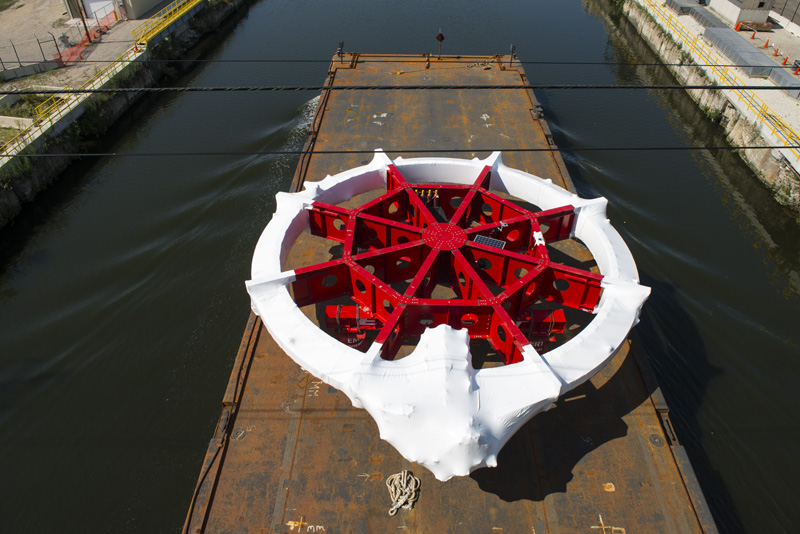
\includegraphics[width=0.8\textwidth]{img/FNAL-13-0232-09D}

%     \hfill\footnotesize [FNAL]
%   \end{center}
% \end{frame}

% \begin{frame}{\insertsection: at Fermilab (FNAL)}
%   \begin{center}
%     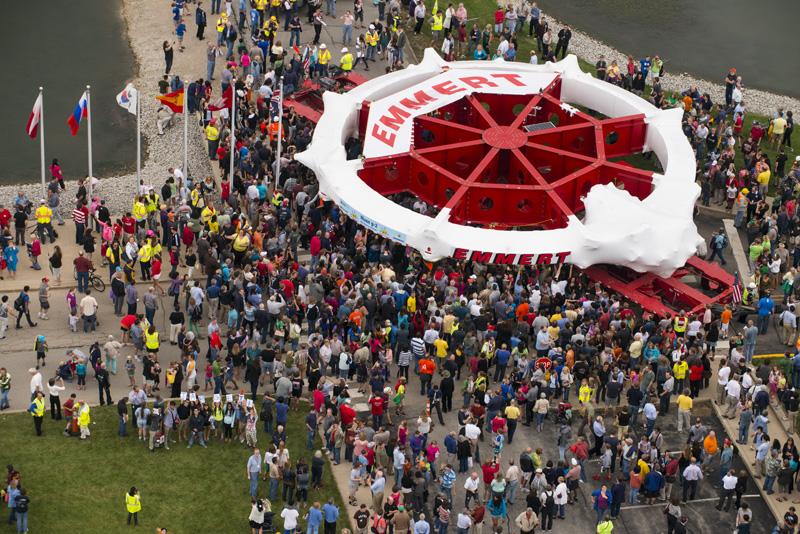
\includegraphics[width=0.8\textwidth]{img/FNAL-13-0244-11D}

%     \hfill\footnotesize [FNAL]
%   \end{center}
% \end{frame}

\begin{frame}{\insertsection: Fermilab (FNAL)}
  \begin{center}
    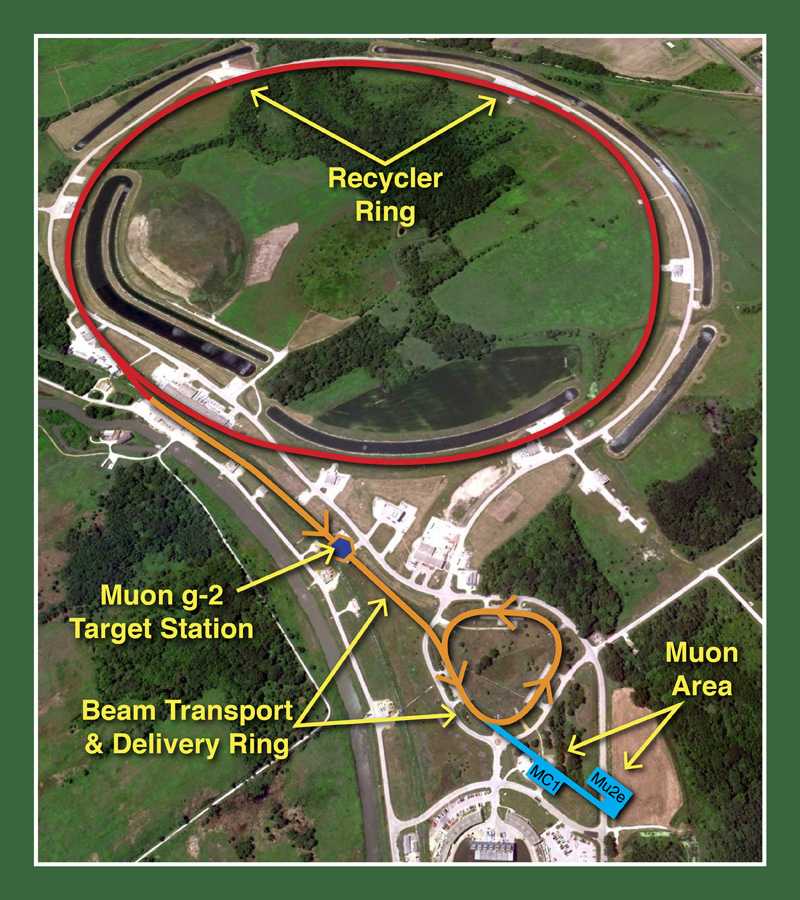
\includegraphics[width=0.7\textwidth]{img/FNAL-14-0280-01D}

    \hfill\footnotesize [FNAL]
  \end{center}
\end{frame}

\begin{frame}{\insertsection: Fermilab (FNAL)}
  \begin{center}
    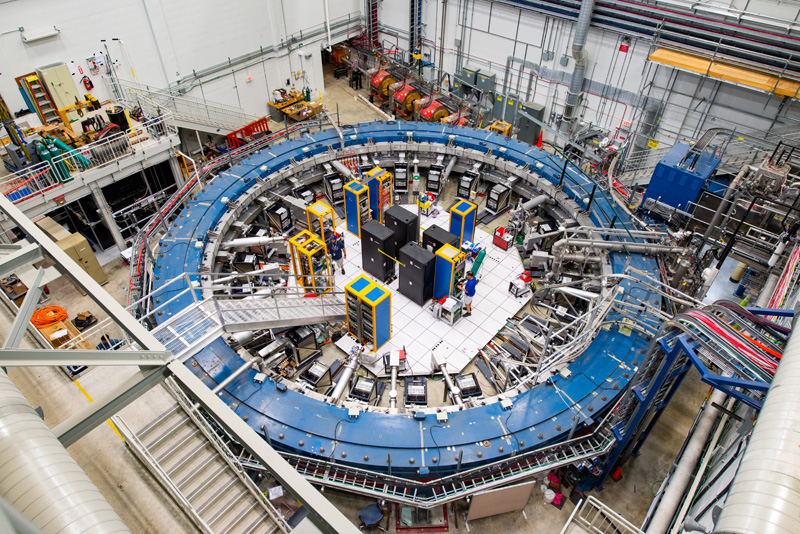
\includegraphics[width=0.9\textwidth]{img/FNAL-17-0188-17}

    \hfill\footnotesize [FNAL]
  \end{center}
\end{frame}

\begin{frame}{\insertsection}
  Exprimental measurements:
  \begin{align*}
    a_\mu^{\text{BNL}} &= (\numamuBNL \pm \DamuBNL)\times 10^{-10} && (2016)\\
    a_\mu^{\text{FNAL}} &= (\numamuFNAL \pm \DamuFNAL)\times 10^{-10} && (2021)
    \intertext{Combined:}
    a_\mu^{\Exp} &= (\numamuExp \pm \DamuExp)\times 10^{-10}
  \end{align*}
\end{frame}

%%%%%%%%%%%%%%%%%%%%%%%%%%%%%%%%%%%%%%%%%%%%%%%%%%

\section{Comparison of measurement and prediction}

% \begin{frame}{\insertsection}
%   \begin{align*}
%     a^{\Exp} &= (\numamuExp \pm \DamuExp)\times 10^{-10} \\
%     a^\SM &= (\numamuSM \pm \DamuSM)\times 10^{-10} \\
%     \Rightarrow\qquad
%     a^{\Exp} - a^\SM &= (25.1 \pm 5.9)\times 10^{-10}
%   \end{align*}
% \end{frame}

\begin{frame}{\insertsection}
  \begin{columns}
    \column{0.7\textwidth}
    \begin{center}
      \begin{tikzpicture}
        \begin{axis}[
          width=\textwidth,
          height=0.8\textheight,
          xlabel = {$(a_\mu - a_\mu^\SM)\times 10^{10}$},
          ymajorticks = false,
          xmin = -10, xmax = 40,
          ymin = 0, ymax = 4,
          ]
          \addplot[blue,dashed,only marks,mark=*,error bars/.cd,x dir=both, x explicit] coordinates {
            (\amuBNL  - \amuSM, 3) +- (\DamuBNL , 0)
            (\amuFNAL - \amuSM, 2) +- (\DamuFNAL, 0)
            % (\amuExp  - \amuSM, 1) +- (\DamuExp , 0)
          };
          \addplot[blue,only marks,mark=*,error bars/.cd,x dir=both, x explicit] coordinates {
            (\amuExp  - \amuSM, 1) +- (\DamuExp , 0)
          };
          \draw[fill,green] (-\DamuSM, 0) rectangle (\DamuSM, 4);
          \node[above] at (\amuBNL  - \amuSM, 3) {BNL};
          \node[above] at (\amuFNAL - \amuSM, 2) {FNAL};
          \node[above] at (\amuExp  - \amuSM, 1) {Experiment};
          \node[black,rotate=90] at (0, 2) {SM prediction};
        \end{axis}
      \end{tikzpicture}
    \end{center}

    \column{0.29\textwidth}
    $a_\mu^{\Exp} - a_\mu^\SM = (25.1 \pm 5.9)\times 10^{-10}$

    \bigskip

    Deviation $\approx 4.2\sigma$

    \bigskip

    % using SpecialFunctions
    % DF(n) = erf(n/sqrt(2))
    % (1 - DF(4.2))*100

    $P(\text{data}|\SM)\approx \num{0.0027}\%$

  \end{columns}
\end{frame}

%%%%%%%%%%%%%%%%%%%%%%%%%%%%%%%%%%%%%%%%%%%%%%%%%%

\section{How can we explain the deviation?}

\begin{frame}{\insertsection}
  Möglicher Grund für Abweichung: Es gibt noch weitere unentdeckte
  Elementarteilchen!
  \begin{itemize}
  \item zusätzliche Higgs-Teilchen?
  \item zusätzliche Quarks oder Leptonen?
  \item Supersymmetrie?
  \end{itemize}
\end{frame}

%%%%%%%%%%%%%%%%%%%%%%%%%%%%%%%%%%%%%%%%%%%%%%%%%%

\section{Open questions}

\begin{frame}{\insertsection}
  \begin{itemize}
  \item Dark Matter
  \item Unification of Forces
  \item Hierarchy Problem
  \end{itemize}
\end{frame}

\end{document}
